%%%% 五号字对应10.5pt
\documentclass[10.5pt]{Template}

\newcommand*\circled[1]{\tikz[baseline=(char.base)]{
            \node[shape=circle,draw,inner sep=1pt] (char) {#1};}}
            
\renewcommand{\baselinestretch}{1.2} 

\newcommand\mycolorRed[1]{{\color{red}#1}}
\newcommand\mycolorYellow[1]{{\color{yellow}#1}}
% \newcommand*\mycolorRed{\color{red}}

\DeclareMathSizes{10.5}{10}{6.8}{4.2}

\setlength{\abovedisplayskip}{2.5mm}
\setlength{\belowdisplayskip}{2.5mm}


\usepackage{tabu}
\usepackage{longtable}
\usepackage{makecell}
\renewcommand\cellgape{\Gape[-3pt][-3pt]}


\begin{document}
\title{
 \erhao\hei 黎曼假设及其证明 
}

\author{
\sihao\kai 王子兴 \\[0.1cm] 
\liuhao (上海交通大学~~数学科学学院,学号~~518070910121) \\ }

\date{}  
\fancyhead[CO]{{\footnotesize 王子兴: 黎曼假设及其证明}}   
\CKeyword{黎曼; 假设; zeta函数; 素数分布}
\CLCNo{V221\makebox{$^{\scalebox{0.6}{\!+}}$}.3;TB553}
\Dcode{A}
\PaperNo{1237-1237 (1237) 66-6666-66}

  \maketitle
\begin{CAbstractJBUAA}
黎曼猜想(或称黎曼假设)是关于黎曼$\zeta$函数$\zeta(s)$的零点分布的猜想,由数学家波恩哈德·黎曼于1859年提出。德国数学家戴维·希尔伯特在第二届国际数学家大会上提出了20世纪数学家应当努力解决的23个数学问题,其中便包括黎曼假设。现今克雷数学研究所悬赏的世界七大数学难题中也包括黎曼假设。
\end{CAbstractJBUAA}

\wuhao 

\section{起源}
\mycolorRed{黎曼猜想}是波恩哈德·黎曼1859年提出的,这位数学家于1826年出生在当时属于汉诺威王国的名叫布列斯伦茨的小镇。1859年,黎曼被选为了柏林科学院的通信院士。作为对这一崇高荣誉的回报,他向柏林科学院提交了一篇题为“论小于给定数值的素数个数”的论文。这篇只有短短八页的论文就是黎曼猜想的“诞生地”。

黎曼论文的一个重大的成果,就是发现了质数分布的奥秘完全蕴藏在一个特殊的函数之中,尤其是使那个函数取值为零的一系列特殊的点对质数分布的细致规律有着决定性的影响。那个函数如今被称为黎曼ζ函数,那一系列特殊的点则被称为黎曼$\zeta$函数的非平凡零点。

有意思的是,黎曼那篇文章的成果虽然重大,文字却极为简练,甚至简练得有些过分,因为它包括了很多“证明从略”的地方。而要命的是,“证明从略”原本是应该用来省略那些显而易见的证明的,黎曼的论文却并非如此,他那些“证明从略”的地方有些花费了后世数学家们几十年的努力才得以补全,有些甚至直到今天仍是空白。但黎曼的论文在为数不少的“证明从略”之外,却引人注目地包含了一个他明确承认了自己无法证明的命题,那个命题就是黎曼猜想。 黎曼猜想自1859年“诞生”以来,已过了161个春秋,在这期间,它就像一座巍峨的山峰,吸引了无数数学家前去攀登,却谁也没能登顶。

有人统计过,在当今数学文献中已有超过一千条数学命题以黎曼猜想(或其推广形式)的成立为前提。如果黎曼猜想被证明,所有那些数学命题就全都可以荣升为定理;反之,如果黎曼猜想被否证,则那些数学命题中起码有一部分将成为陪葬。

\section{黎曼假设原题的证明}
\subsection{预备知识}
\subsubsection{一个行列式相关的引理}
Given two subspaces $U$ and $V$ in an Euclid space $\mathbb{R}^n$, then we can define the angle between $U$ and $V$ as the minimum angle between $u$ and $v$ for all $u\in U$, $v\in V$, namely $\theta\left(U,V\right)=min\left\{\theta\left(u,v\right)\right\}$.

Let $A$ be an $r$ by $n$ matrix and $B$ be an $s$ by $n$ matrix. Orthonormalize $A$ into $A'$ and $B$ into $B'$. The cosine of the angle between the the column space of $A$ and the column space of $B$ is equal to $\sigma_{1}$, where $\sigma_{1}$ is the biggest singular value of $A'^{T}B'$.\citeBUAA{AA,FF}
\subsubsection{DNA对黎曼假设的影响}
脱氧核糖核酸(英文DeoxyriboNucleic Acid,缩写为DNA)是生物细胞内含有的四种生物大分子之一核酸的一种。

DNA携带有合成RNA和蛋白质所必需的遗传信息,是生物体发育和正常运作必不可少的生物大分子。

DNA由脱氧核苷酸组成的大分子聚合物。脱氧核苷酸由碱基、脱氧核糖和磷酸构成。其中碱基有4种:腺嘌呤(A)、鸟嘌呤(G)、胸腺嘧啶(T)和胞嘧啶(C)。

DNA 分子结构中,两条多脱氧核苷酸链围绕一个共同的中心轴盘绕,构成双螺旋结构。脱氧核糖-磷酸链在螺旋结构的外面,碱基朝向里面。两条多脱氧核苷酸链反向互补,通过碱基间的氢键形成的碱基配对相连,形成相当稳定的组合。

由此可见,DNA至关重要。

\begin{figure}[h!]
\centering
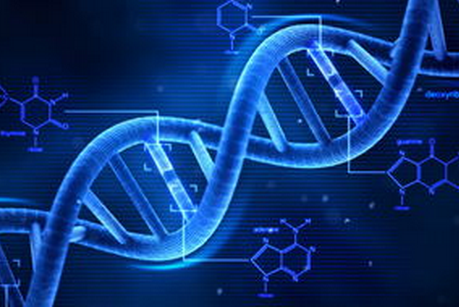
\includegraphics [scale=0.3,trim=0 0 0 0]{./image/dna.png}
\caption{DNA对黎曼假设的影响}
 \label{DNA}
\end{figure}

\section{结~~论}
根据前面的说明,我们得到以下结论:

1) 黎曼假设需要非方阵行列式的背景才能证明。

2) 另外,DNA的结构也对黎曼假设的证明起到了至关重要的作用。


%  参考文献

\renewcommand\refname{\hei\wuhao\centerline{参考文献(References)}\global\def\refname{参考文献}}
\vskip 12pt

\let\OLDthebibliography\thebibliography
\renewcommand\thebibliography[1]{
  \OLDthebibliography{#1}
  \setlength{\parskip}{0pt}
  \setlength{\itemsep}{0pt plus 0.3ex}
}

{
\renewcommand{\baselinestretch}{0.9}
\liuhao
\bibliographystyle{unsrt}
\bibliography{./TempExample}
}


% 作者简历
{
\xiaowuhao
\noindent {\hei 作者简介:}

\noindent {\hei 王子兴}~~~ 男,本科生。主要研究方向:黎曼假设与物质的拓扑相变和拓扑相的关系。
\vskip 16pt

\end{document}
